\subsection{Extension for team time trial}
\par Team time trial (TTT) is generally composed of six drivers as a team, and the fourth-place finisher in the team will be the team result. Teams generally use a straight-line formation, with a gap of 30-50 cm between riders, so that the rider at the front can block the wind for others behind. When the team is moving at a constant speed, the required output power per kilogram decreases from the head of the row to the end [\ref{beauty}], as does the energy per kilogram required to complete a unit of distance.
% TODO: \usepackage{graphicx} required
\begin{figure}[h]
	\centering
	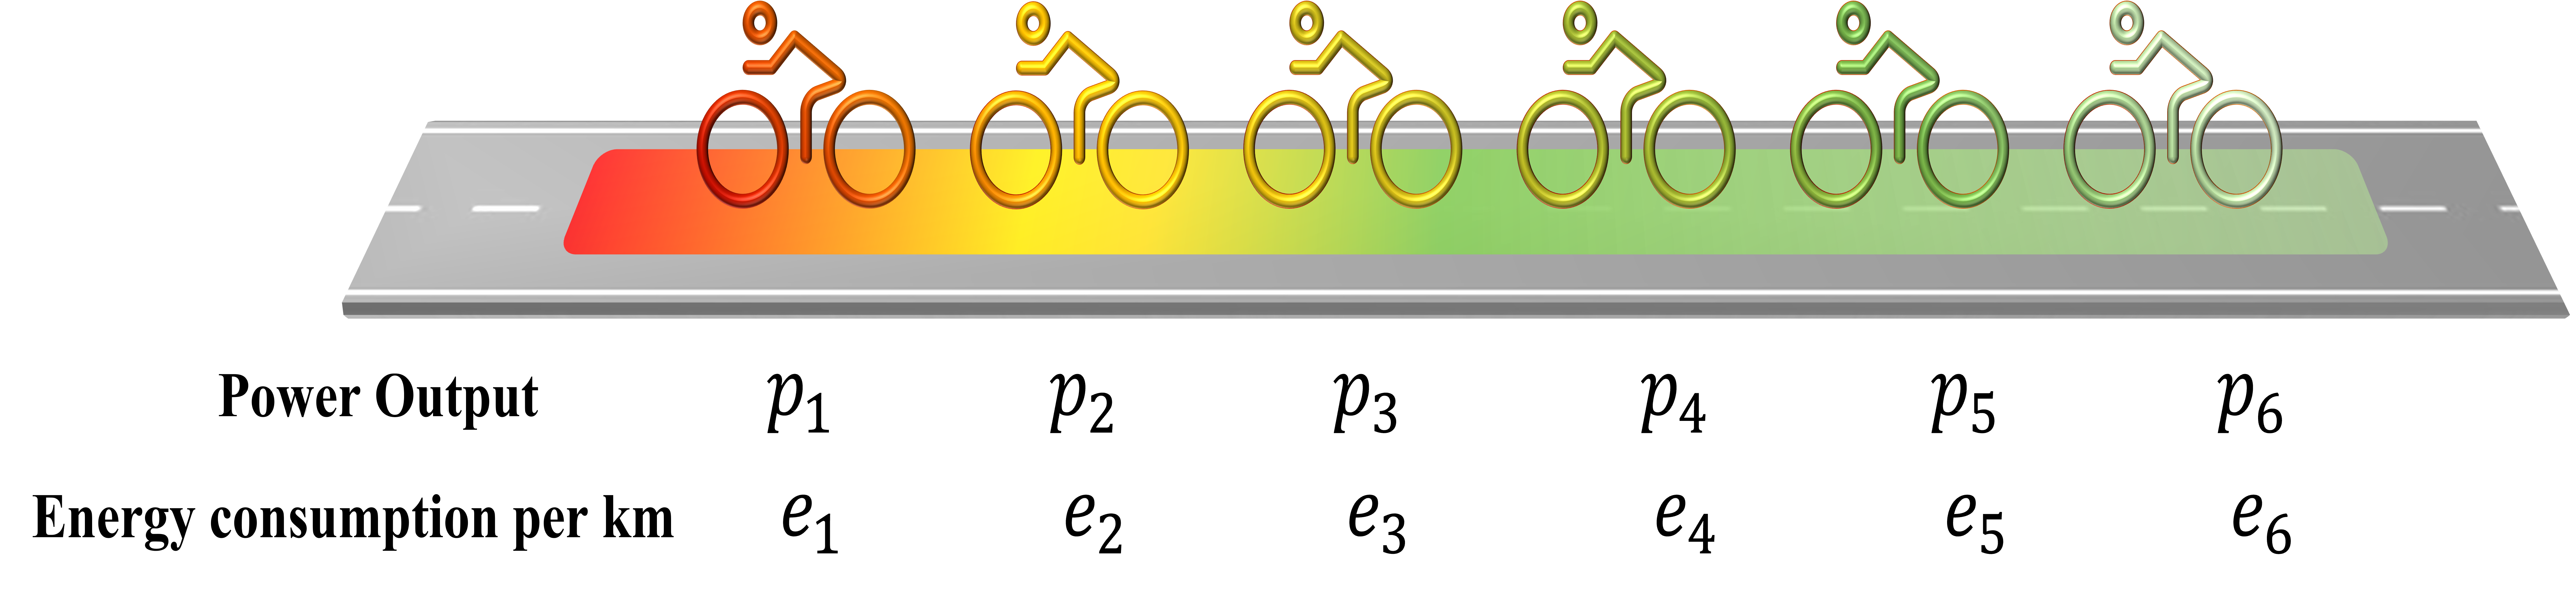
\includegraphics[width=1\linewidth]{image/beauty}
	\caption{Team time trialist diagram}
	\label{beauty}
\end{figure}

\par After watching some races, we find that teams generally have only four riders when they are approaching the finish line, leaving the remaining two far behind due to lack of energy. When we extend the model to team time trial, the six drivers shall be split into a stronger four and a weaker two, which will fall behind in the race.

\par In our model extension, riders in the team take turns taking the lead to block the wind and move forward at a constant speed $\nu$. The entire race process is divided into three stages, with 6, 5, and 4 riders making up the team respectively, and each stage consists of several same leading cycles. A leading period refers to the period from when a rider leaves the lead position to the next lead.

\par Let $\sigma_j(j\leq3)$ be the track of stage $j$, $p_i(i\leq6)$ be the power output per kilogram of the $i^{th}$ position in formation, and $e_i(s)(i\leq6)$ be the cost of energy per kilogram to complete 1 km. Moreover, $N_j$ is used to denote the number of leading cycles with length $T_j$ included in stage $j$.

\par This way, we can list the corresponding PTE equations for each stage: 

\begin{equation}\label{PTEeqs}
	\begin{split}
		\left\{
	\begin{aligned}
	N_1p_1T_1 &=\sum_{i=1}^{6}\int_{\sigma_1}e_i(s)ds  \\
	N_2p_2T_2 &=\sum_{i=1}^{5}\int_{\sigma_2}e_i(s)ds  \\
	N_3p_3T_3 &=\sum_{i=1}^{4}\int_{\sigma_3}e_i(s)ds  
	\end{aligned}
	\right.
\end{split}
\end{equation}

\par and the following constraints:

\begin{equation}\label{teamcons}
\begin{split}
		\left\{
		\begin{aligned}
	&(N_1-1)T_1<f_6^{-1}(p_6)\leq N_1T_1 \\
	&(N_2-1)T_2<f_5^{-1}(p_5)+N_1T_1\leq N_2T_2 \\
	&N_3T_3 \leq f_4^{-1}(p_4)
\end{aligned}
\right.
\end{split}
\end{equation}

\par where $f_i$ is the power curve of $i^{th}$ most energetic and powerful rider in the team.

\par Constraints (\ref{teamcons}) point out when the two weakest players in the team will be exhausted and fall behind. And we can give the best strategy for the team by solving an optimization problem similar to (\ref{min})(\ref{cons3})  in our PTE model:

\begin{equation}
	\min N_1T_1+N_2T_2+N_3T_3 \quad\quad \rm{s.t.}
\end{equation}

\begin{equation}
\begin{split}
	\left\{
	\begin{aligned}
	&N_jp_jT_j =\sum_{i=1}^{7-j}\int_{\sigma_j}e_i(s)ds,j=1,2,3\\
	&(N_1-1)T_1<f_6^{-1}(p_6)\leq N_1T_1 \\
	&(N_2-1)T_2<f_5^{-1}(p_5)+N_1T_1\leq N_2T_2 \\
	&N_3T_3 \leq f_4^{-1}(p_4)
\end{aligned}
		\right.
\end{split}
\end{equation}

\par Of course, PTE model for TTT can take into account more factors, such as considering the movement of the team as a speed change motion, and considering environmental factors such as weather and slope, so as to induce the expression of $e_i(s)$. At the same time, we can also establish the relationship between $p_i$ and $e_i$ through the speed $\nu$. Although these works require more computational resources and data, they can all be refined within the framework of our PTE model.
